\section{Compact Torus (CT)}
\begin{frame} {Starting From Nuclear Fusion}
    In order to make fusion energy a viable economic alternative, significant improvements in concept design need to occur.
    \begin{itemize}
        \item We want the device to be \textbf{Simply connected}. Meaning that there is no material linking the center of the device, making the first wall either a sphere or a cylinder.
        \item By removing the center material of the device, the cost decreases and the engineering becomes simple.
        \item Compact Torus suits this purpose very well.
    \end{itemize}
\end{frame}

\begin{frame} {Well Studied CTs}
    \begin{itemize}
        \item Compact torus is a toroidal magnetic configuration with a simply-connected geometry that are self-stable.
    \end{itemize}

    The following configurations fall into the category of compact torus:
    \begin{itemize}
        \item Spheromak.
        \item Field-reversed configuration (FRC).
        \item Particle ring. (Not in active research today.)
    \end{itemize}
\end{frame}

\begin{frame} {Spheromak}
    \begin{itemize}
        \item Spheromak is a toroidal confinement with toroidal and poloidal fields.
        \item Toroidal field is completely generated by plasma currents.
        \item The current is toroidal at the core and poloidal at the surface.
        \item The current is parallel to $\mathbf{B}$ in spheromak, $\grad p = \mathbf{j\times B}=0$.
        \item Ideally it is always MHD stable. In reality, spheromak has finite pressure and due to different decay rates of toroidal and poloidal fields, current driven kink modes will be developed.
    \end{itemize}

    \begin{figure}
        \centering
        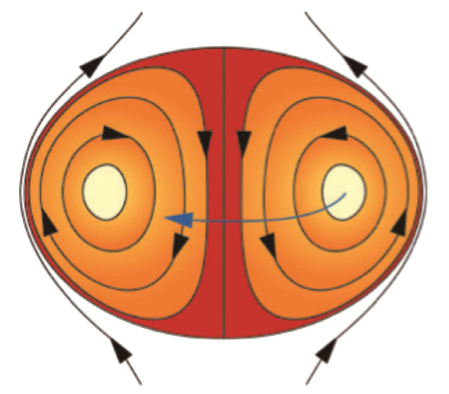
\includegraphics[width=0.3\textwidth]{figures/sphromak.png}
        \caption{Spheromak configuration. \cite{gao_2016_compact} The arrow lines are magnetic field lines.}
        \label{fig:spheromak}
    \end{figure}

    \tiny \cite{gao_2016_compact} Z.Gao. \textit{Compact magnetic confinement fusion: Spherical torus and compact torus.}
\end{frame}

\begin{frame} {Spheromak Issues \cite{gao_2016_compact}}
    \begin{itemize}
        \item Due to absence of toroidal field coils, it is difficult to generate large toroidal fields in spheromak.
        \item Due to absence of ohmic coils, it is difficult to obtain long pulse discharges.
        \item The above issues indicates: it is hard to achieve good confinement simultaneously with an efficient current drive. The drive of plasma current will break the magnetic surface and induce high-level heat losses.
    \end{itemize}
\end{frame}

\begin{frame} {Spheromak Successes \cite{woodruff_2008_technical}}
    \begin{itemize}
        \item Tokamak-like transport measured in the SSPX experiment by suppressing fluctuations.
        \item Multi-pulsed build-up of magnetic energy in a spheromak demonstrated in SSPX.
        \item SSX merged spheromaks and detailed magnetic reconnection and generation of energetic plasma flows, FRC formation by merging.
        \item TS-3/4 shows means for forming various toroidal configurations by merging.
    \end{itemize}
\end{frame}

\begin{frame} {Field Reversed Configuration (FRC)}
    \begin{itemize}
        \item FRC is a toroidal confinement with poloidal field only.
        \item Bulk currents of FRC are diamagnetic, leading to a high beta $\sim$ 1.
        \item FRC equilibrium cannot be described by Grad-Shafranov equation. Two-fluid or kinetic theory is needed.
        \item FRC's magnetic topology indicates that it is unstable to most ideal MHD modes, but robust stability can be obtained in experiments.
    \end{itemize}

    \begin{figure}
        \centering
        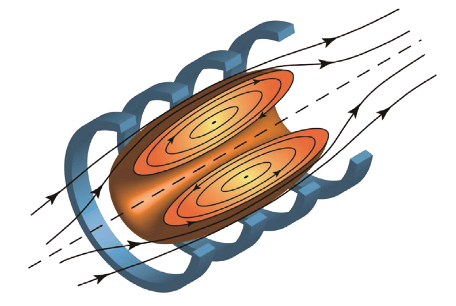
\includegraphics[width=0.3\textwidth]{figures/frc.png}
        \caption{Field reversed configuration. \cite{gao_2016_compact} Arrow lines are magnetic field lines.}
        \label{fig:frc}
    \end{figure}

    \tiny \cite{gao_2016_compact} Z.Gao. \textit{Compact magnetic confinement fusion: Spherical torus and compact torus.}
\end{frame}

\begin{frame} {FRC Issues \cite{gao_2016_compact}}
    \begin{itemize}
        \item It is believed that Finite Larmor radius (FLR) effect contributes to the stability, but this effect is not effective in large-size FRC.
        \item Sheared flows and large orbit of energetic ions may improve stability but theoretical explanations and experimental evidences are not well convincing.
        \item FRC provides a big challenge in equilibrium and stability of plasmas at the extreme.
    \end{itemize}
\end{frame}

\begin{frame} {FRC Successes \cite{woodruff_2008_technical}}
    \begin{itemize}
        \item Formation and Sustainment of long-lived FRCs in the TCS device (10 ms).
        \item Production of low-density FRCs with enhanced confinement in Osaka FIX experiment.
        \item Production of high density FRCs in the FRX-L device. FRCs have been formed with an equilibrium density $n_e (\sim 1-2) 10^{16}$\unit{\cm^{-3}}, $T_e < T_i \sim 250$\unit{eV}, and excluded flux $2-3$\unit{\milli\weber}.
        \item Formation, acceleration to $M > 1$, and collisions of FRCs in the IPA device.
    \end{itemize}
\end{frame}

\begin{frame} {Comparison Among Configurations}
    \begin{itemize}
        \item CT can be used in fusion technology.
    \end{itemize}
    \begin{figure}
        \centering
        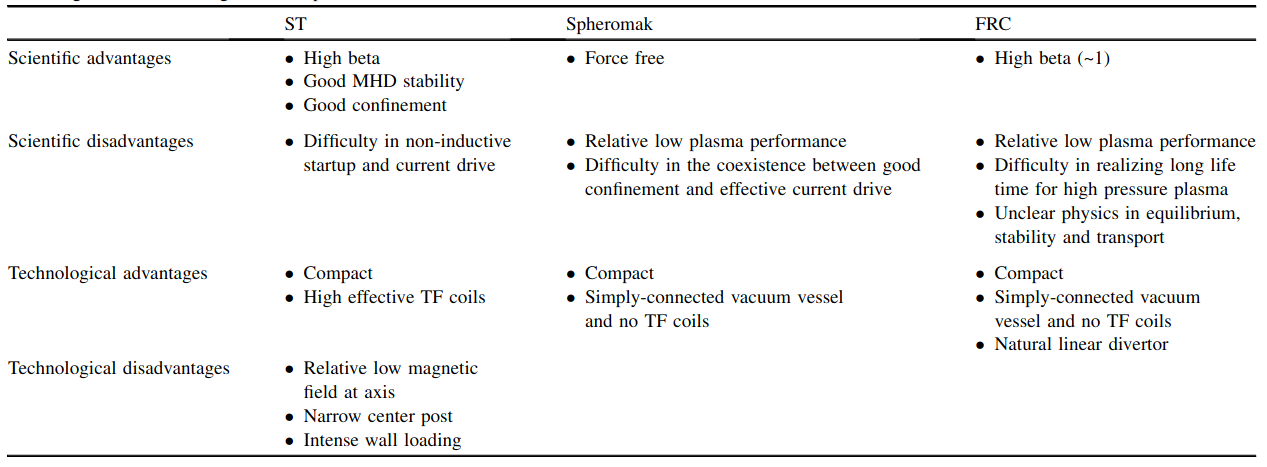
\includegraphics[width=\textwidth]{figures/comparisons.png}
        \caption{Advantages and disadvantages of Spherical Tokamak (ST), spheromak and FRC for fusion. \cite{gao_2016_compact}}
        \label{fig:comparisons}
    \end{figure}

    \tiny \cite{gao_2016_compact} Z.Gao. \textit{Compact magnetic confinement fusion: Spherical torus and compact torus.}
\end{frame}

\begin{frame} {Plasma Performance Achievements}
    \begin{figure}
        \centering
        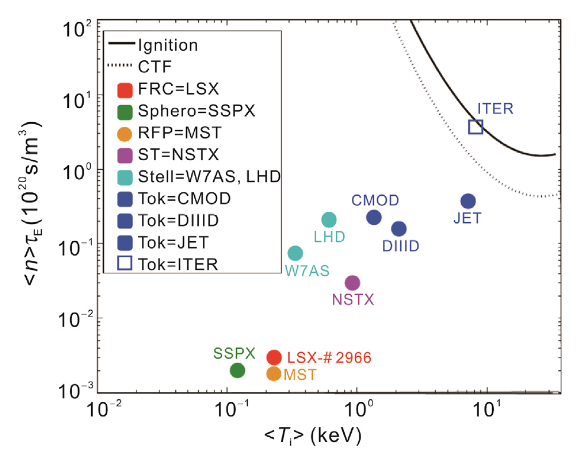
\includegraphics[width=0.7\textwidth]{figures/plasma-performance.png}
        \caption{Plasma performance achievements of various concepts. \cite{gao_2016_compact}}
        \label{fig:plasma-performance}
    \end{figure}

    \tiny \cite{gao_2016_compact} Z.Gao. \textit{Compact magnetic confinement fusion: Spherical torus and compact torus.}
\end{frame}